\documentclass[Main]{subfiles}

\begin{document}
\section{Results and Discussion}
This project has implemented the function \texttt{miniproject(t\_errors, errorloc)} in Matlab which runs the cyclic encoder and Meggitt decoder.
The function will return 1 if the messages has been decoded into a correct code word, otherwise it will return 0.
It takes the parameters \texttt{t\_errors}, which is the number of errors which should be added to the message, and \texttt{errorloc} which is the location of the errors.
If \texttt{errorloc} is not used the error location(s) will added randomly, and if \texttt{t\_errors} is not used 2 errors at random locations will be introduced. 

Some screen dumps form Matlab calling the \texttt{miniproject()} function will be discussed in the following.

The result form calling the function introducing one error is shown in Figure \ref{fig:result-1-errors}.
It can be seen that the codeword has been decoded successfully.
Furthermore it shows the different vectors and the tag telling what the Meggitt decoder has done. 

\begin{figure}[h!]
\centering
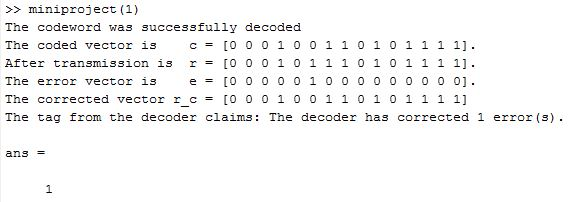
\includegraphics[width=0.7\linewidth]{./Picture/result-1-errors}
\caption{Meggitt decode run with one error, no location}
\label{fig:result-1-errors}
\end{figure}

The Figures \ref{fig:result-2-errors}, \ref{fig:result-2-errors-location} and \ref{fig:result-3-errors} shows the results of other inputs:

In Figure \ref{fig:result-3-errors} it is seen that it is possible to detect, that there is more than 2 errors but the decoder is not able to correct it. 

\begin{figure}[h!]
\centering
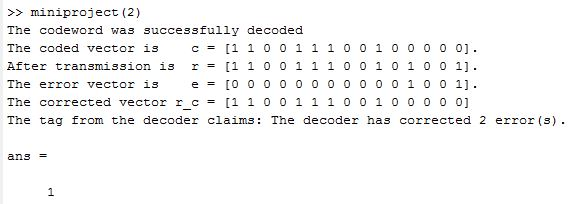
\includegraphics[width=0.7\linewidth]{./Picture/result-2-errors}
\caption{Meggitt decoder run with two errors, no location}
\label{fig:result-2-errors}
\end{figure}

\begin{figure}[h!]
\centering
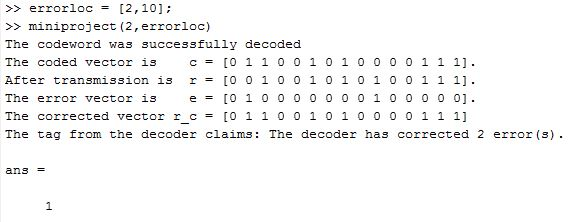
\includegraphics[width=0.7\linewidth]{./Picture/result-2-errors-location}
\caption{Meggit decoder run with 2 errors, with location}
\label{fig:result-2-errors-location}
\end{figure}

\begin{figure}[h!]
\centering
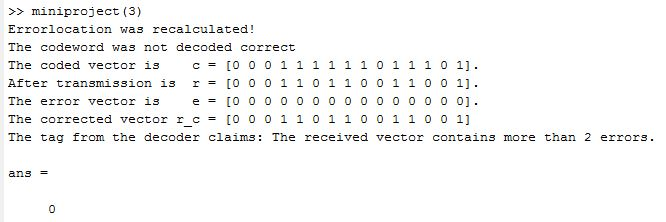
\includegraphics[width=0.7\linewidth]{./Picture/result-3-errors}
\caption{Meggitt decoder run with 3 errors, no location}
\label{fig:result-3-errors}
\end{figure}

Carrying out this project, all the encoding and decoding procedures have been calculated by hand simultaneous with the Matlab code development.
The calculations in hand have been done to ensure that the Matlab codes have been developed in the right way.
A codes has been generated and tested in Matlab and by hand as well, and the results have been matched.
When the results differed the procedures have been checked and errors have been corrected.

The function \texttt{miniproject(t\_errors, errorloc)} is able to correct 1 and 2 errors in a codeword, which can be seen in Figure \ref{fig:result-1-errors}, \ref{fig:result-2-errors} and \ref{fig:result-2-errors-location}.

It is also possible to detect more than 2 errors.
When introducing 3 errors it is not possible to correct them, but the Meggitt decoder is able to detect that there is more than 2 errors, see Figure \ref{fig:result-3-errors}.\\

It is possible to introduce a codeword with 3 errors, which can be corrected into a valid codeword.
At first this gave some frustration until putting some deeper thoughts into this.
A possible cause to this could be that when introducing 3 errors to a codeword this can result in a codeword with only 2 errors, which the function is able to correct to a valid codeword.

This can be explained as follows:
The general polynomial has a weight of 5 which give a $d_{min}=5$.
When only introducing 2 or less errors it is sure that the shortest distance is to the correct codeword.
When introducing 3 or more errors, there is a possibility that it is getting a distance of two to an other codeword.
In the way the \texttt{miniproject(t\_errors, errorloc)} has been implemented it will always look for the codeword with the shortest distance, which it is why it will reach a valid but wrong codeword.
This might be corrected in the code so when 1 error has been found the decoder knows that if there should be another error it should be when there is only one error in the rightmost bit.
So by minimizing the error pattern table when an error has been detected ensures that the function does not use the error pattern for 2 errors twice.
This is not implemented in Matlab, but would be a next step to go. 



\end{document}
